\section{Dataset Preparation}
In this project, we use the \href{https://www.kaggle.com/datasets/skylarkphantom/mit-datacenter-challenge-data?select=scheduler_data.csv}{MIT Supercloud dataset}. Generally speaking, a High Performance Computing (HPC) system consists of a number of nodes. When a user submits a task, it is pushed to a queue. A scheduler decides how many nodes are assigned to the next task in the queue based on the number of available nodes. When a task is allocated with some nodes, it begins executing. After execution, the nodes are recollected. Hence there are three time points worth noticing, namely submitting time, start time and end time.

We consider the following features in the MIT Supercloud dataset
\begin{itemize}
  \item \texttt{nodes\_alloc}: the number of nodes allocated to a task.
  \item \texttt{time\_submit}: the time stamp in seconds when a user submits a task.
  \item \texttt{time\_start}: the time stamp in seconds when a task starts executing.
  \item \texttt{time\_end}: the time stamp in seconds when a task executed.
\end{itemize}

Assuming that all nodes have the same computing power, we calculate a temporary feature $$\texttt{task\_complexity} = (\texttt{time\_end} - \texttt{time\_start})\times \texttt{nodes\_alloc}.$$

Once having the number of nodes and time complexity, we can calculate back the time needed to execute. Our raw training data consists of \texttt{time\_submit} and \texttt{task\_complexity} features. We aim to minimize
$$\texttt{time\_wait} = \texttt{time\_start} - \texttt{time\_submit}.$$

Due to computation limit, training and inferring for every second is intractable. The best practice for an experimental project is to train and infer hourly.

\begin{figure}[ht]
  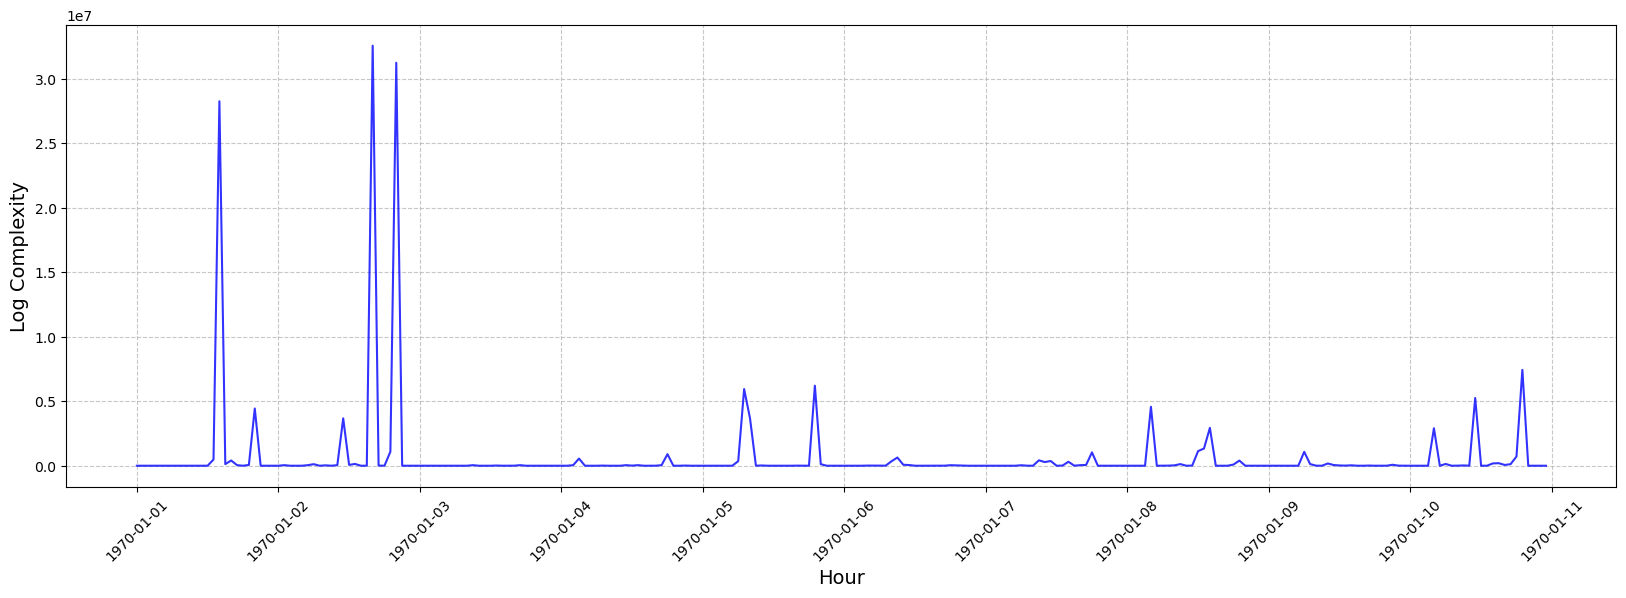
\includegraphics[width=\textwidth]{img/hourly.png}
\end{figure}